% !TEX root= ../main.tex
\externaldocument{discoursegraphs}
\externaldocument{kerneltheory}
\section{Resolving GNF-theories}
\label{sec:Resolving GNF-theories}
In this section, I present an inference system introduced by Walicki in \cite{michal-completeness} which reasons over clausal theories induced from GNF-theories.
The system is refutationally complete as well as non-explosive, allowing us to identify consistent parts of paradoxical discourse theories.

We later show some correlations between certain graph structures and clauses provable in this inference system.

Recall that a GNF theory consists exclusively of formulae of the following form:
\begin{align}
  x \lar \bigwedge_{i \in I_x} \neg y_i
\end{align}
Using simple operations only, these formulae can be translated into an equivalent set of clauses.
We start by writing the above bi-implication as two implications:
\begin{align}
  x \rightarrow \bigwedge_{i \in I_x} \neg y_i \quad\quad \text{and} \quad\quad x \leftarrow \bigwedge_{i \in I_x} \neg y_i
\end{align}
The first implication can be rewritten in the following way:
\begin{align}
  x \rightarrow \bigwedge_{i \in I_x} \neg y_i
  \quad\Leftrightarrow\quad \neg x \vee \bigwedge_{i \in I_x} \neg y_i
  \quad\Leftrightarrow\quad \bigwedge_{i \in I_x} (\neg x \vee \neg y_i)
  \quad\Leftrightarrow\quad \bigwedge_{i \in I_x} \neg (x \wedge y_i)
\end{align}
The second implication can be rewritten in the following way:
\begin{align}
  x \leftarrow \bigwedge_{i \in I_x} \neg y_i
  \quad\Leftrightarrow\quad x \vee \neg \left( \bigwedge_{i \in I_x} \neg y_i \right)
  \quad\Leftrightarrow\quad x \vee \bigvee_{i \in I_x} y_i
\end{align}
By splitting the conjunction from the first implication up into individual clauses, we get the following two kinds of clauses for every variable $x$ in the GNF theory:
\begin{align}
  \text{OR-clause:}&\quad x \vee \bigvee_{i \in I_x} y_i\\
  \text{NAND-clauses:}&\quad \neg (x \wedge y_i)\text{, for every }i \in I_x
\end{align}
We will treat both the OR-clauses and the NAND-clauses as sets of atoms, denoting NAND-clauses $\neg (x \wedge y)$ as $\overline{xy}$ and OR-clauses $x \vee y_1 \vee y_2 \vee y_3$ as $xy_1y_2y_3$.
This enables us to state things like $\overline{xy} \subset \overline{xyz}$.
A theory will -- as expected -- be a set of OR- and NAND-clauses.

If we interpret the initial GNF-theory as a graph $\mathbf{G}=\langle G,N\rangle$, for every vertex $x \in G$, there will be one OR-clause $\{ x \} \cup N(x)$ and for every edge $\langle x,y \rangle \in N$ there will be a NAND-clause $\overline{xy}$.

The graphs from Figure~\ref{ex:3graphs} will have the following clausal theories:
\begin{align}
  \mathcal{T}(\mathbf{G_1}) &= \{ a, \ol{a} \}\\
  \mathcal{T}(\mathbf{G_2}) &= \{ abc, b, c, \ol{ab}, \ol{ac} \}\\
  \mathcal{T}(\mathbf{G_3}) &= \{ abc, bc, \ol{ab}, \ol{bc} \}
\end{align}
Further notation: $A\subseteq G$ denotes an OR-clause while $\ol{A} \subseteq G$ denotes a NAND-clause.
Given a graph $\mathbf{G}=\langle G,N\rangle$, we denote the set of all NAND-clauses induced from the graph as NAND and all induced OR-clauses as OR.
The combined set $\Gamma = NAND + OR$ will be our initial clauses in the inference system.
\subsection{The inference system}
\label{sub:The inference system}
We consider the following inference system, but we will focus mainly on proofs using the Axioms together with the (Rneg) rule.
\begin{align}
  \text{(Ax)} &\quad \Gamma \vdash C, \quad \text{for } C \in \Gamma\\
  \text{(Rneg)} &\quad \frac{ \{ \Gamma \vdash \ol{a_iA_i} \; |\; i \in I \} \quad \Gamma \vdash \{ a_i \; |\; i \in I \} }{ \Gamma \vdash \ol{\bigcup_{i \in I} A_i} }\\
  \text{(Rpos)} &\quad \frac{ \Gamma \vdash A \quad \{\Gamma \vdash B_iK_i \; |\; i \in I \} \quad \{ \Gamma \vdash \ol{a_ik} \; |\; i \in I, k \in K_i \} }{ \Gamma \vdash (A \setminus \{ a_i \; |\; i \in I \} ) \cup \bigcup_{i \in I} B_i }
\end{align}
(Rneg) is creating NAND-clauses from NAND-clauses using OR as a side-condition.
(Rpos) is creating OR-clauses from OR-clauses using NAND as a side-condition.
In (Rneg), $\ol{a_iA_i}$ denotes the NAND $\ol{\{ a_i \} \cup A_i}$ with a potentially empty $A_i$.

A proof in this system is a well-founded derivation, i.e. each of the branches in the proof tree is finite.
This allows us to induce over the complexity of the proof tree.

The premise of the (Rneg)-rule is a set of $I$ NAND-clauses together with one OR-clause with $I$ elements such that each atom $a_i$ in the OR-clause is contained within a NAND-clause, and such that each NAND-clause contains an atom from the OR-clause.
The correspondence between the NAND-clauses and the elements of the OR-clause should in other words be bijective.
The conclusion is the union of all the NAND-clauses without their corresponding atom from the OR-clause.

Whenever it is obvious and/or irrelevant from what theory we are proving something, we leave out this information in the proof to ease readability.
Additionally, we move the single OR-clause in the premise to the side of the proof to emphasize its role as a side condition.
These conventions are illustrated below:\par
\begin{figure}[!h]
  \centering
  \begin{prooftree}
    \Hypo{\Gamma \vdash \ol{ax} }
    \Hypo{\Gamma \vdash \ol{by} }
    \Hypo{\Gamma \vdash ab}
    \Infer[]3{\Gamma \vdash \ol{xy}}
  \end{prooftree}
  \hspace{2mm} $\sim$ \hspace{2mm}
  \begin{prooftree}
    \Hypo{\ol{ax}}
    \Hypo{\ol{by}}
    \Infer[right label = $ab$]2{\ol{xy}}
  \end{prooftree}
  \caption{}
  \label{fig:proof_convention}
\end{figure}
Here are some examples of incorrect applications of the (Rneg)-rules, followed by some correct applications:
\begin{align}
  (1)\;\;\frac{\ol{ax}\quad\ol{by}\quad\ol{cz}}{\ol{xyz}}abx\quad\quad
  (3)\;\;\frac{\ol{ax}\quad\ol{by}}{\ol{xy}}abx\quad\quad
  (2)\;\;\frac{\ol{ax}\quad\ol{by}\quad\ol{bz}}{\ol{xyz}}abx
\end{align}
(1) is incorrect because the NAND $\ol{cz}$ contains no atoms from the OR $abx$.
(2) is incorrect because the number of NAND-clauses does not match the length of the OR-clause.
(3) is incorrect because there exist no bijective correspondence of the type described above.
\begin{align}
  (4)\;\;\frac{\ol{ax}\quad\ol{by}\quad\ol{cz}}{\ol{xyz}}abc\quad\quad
  (5)\;\;\frac{\ol{ax}\quad\ol{b}}{\ol{x}}ab\quad\quad
  (6)\;\;\frac{\ol{ax}\quad\ol{by}\quad\ol{xyz}}{\ol{xyz}}abx
\end{align}
The above applications are all correct, since all the atoms in each OR-clause get matched to exactly one NAND-clause in such a way that no NAND-clause stays unmatched.

The proof system sets no restrictions on the number and cardinality of its clauses, meaning that there might be an infinite number of clauses, and both the OR-clauses and the NAND-clauses might be either finite or infinite in size.
Note that an infinite graph gives infinitely many NAND- and OR-clauses, while an infinitary graph also gives us infinitely \textit{long} OR-clauses.

We study the refutation system that arises from the axioms and the (Rneg)-rule, calling it Neg.
It is shown in \cite{michal-completeness} that Neg is sound for arbitrary theories and refutationally complete for theories with a countable number of OR-clauses.
Soundness gives us for any graph $\mathbf{G} = \langle G,N \rangle$ that proving $\ol{C}$ for any $C \subseteq G$ implies that the vertices in $C$ cannot all be assigned 1 in the graph model $\mathcal{T}(\mathbf{G})$.
Refutational completeness gives us the property that whenever a graph/theory is inconsistent, we are able to prove $\varnothing$ in Neg.

We use the notation $\Gamma \vDash \ol{C}$ to express that every model of the theory $\Gamma$ satisfies the NAND-clause $\ol{C}$.
Note that because of the model/kernel equivalence presented in Section~\ref{sec:Discourse Theories and Digraphs}, the notation can also be used to express that none of the kernels in the graph $\mathcal{G}(\Gamma)$ contains all the vertices in the set $C$.

Since refutational completeness is only proven for theories with countably many OR-clauses, this thesis will only consider graphs with a countable number of vertices.
We are thus able to assume both soundness and refutational completeness for all following graph theories.

Note that Neg is not generally complete, i.e. we do not always have that $G\vDash {x} \; \Rightarrow \; G \vdash \ol{x}$.
The inconsistent graph $G$ in Figure~\ref{fig:neg_not_complete} exemplifies this:\par
\begin{figure}[!h]
  \centering
  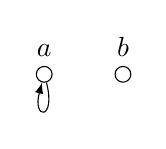
\begin{tikzpicture}
    [
    point/.style={circle,draw,inner sep=0pt,minimum size=2mm}
    ]
    \node (1) at (0,0) [point, label=above:$a$] {};
    \node (2) at (1,0) [point, label=above:$b$] {};
    \draw [-latex, loop below] (1) to (1);
  \end{tikzpicture}
  \caption{}
  \label{fig:neg_not_complete}
\end{figure}
\FloatBarrier
Because of the loop on vertex $a$, the graph has no solutions.
We therefore have $G \vDash \varnothing$ and thus also $G \vDash \ol{b}$, but we are unable to prove $\ol{b}$ in Neg.
\subsection{Inconsistency of the Yablo-graph}
\label{sub:Inconsistency of the Yablo-graph}
The inconsistency of the Yablo-graph is easily proven using Neg only.
Since every vertex $x_i$ (using the notation from Figure~\ref{fig:yablo-graph}) has an edge to each vertex $x_j$ where $j > i$, we get that every pair of distinct vertices is connected by an edge.
This means that our set of axioms from the Yablo-graph looks like this:
\begin{align}
  \text{NAND} = \{ \ol{x_ix_j} \; |\; i < j\}
  \quad\quad\quad
  \text{OR} = \{ x_ix_{i+1}x_{i+2}\dots \; |\; i \in \mathbb{N}\}
\end{align}
For any vertex $x_i$ from the Yablo-graph, we are now able to prove $\ol{x_i}$ in the following way:\par
\begin{figure}[!h]
  \centering
  \begin{prooftree*}
    \Hypo{\ol{x_ix_{i+1}}}
    \Hypo{\ol{x_ix_{i+2}}}
    \Hypo{\ol{x_ix_{i+3}}}
    \Hypo{\dots}
    \Infer4[$x_ix_{i+1}x_{i+2}\dots$]{\ol{x_i}}
  \end{prooftree*}
  \caption{}
  \label{fig:proof_xi}
\end{figure}
Proving $\varnothing$ is now simple:\par
\begin{figure}[!h]
  \centering
  \begin{prooftree*}
    \Hypo{\dots}
    \Infer1{\ol{x_1}}
    \Hypo{\dots}
    \Infer1{\ol{x_2}}
    \Hypo{\dots}
    \Infer1{\ol{x_3}}
    \Hypo{\dots}
    \Infer4[$x_1x_2x_3\dots$]{\varnothing}
  \end{prooftree*}
  \caption{}
  \label{fig:proof_yablo}
\end{figure}
A less trivial inconsistency proof is the one of the \textit{Stretched Yablo-graph}.
This proof can be found in Appendix~\ref{sec:Inconsistency of Stretched Yablo} together with the definition of Stretched Yablo.

It is worth mentioning that even though our focus has been -- and will be -- on theories originating from graphs, the results on soundness and completeness hold for any theory consisting of a set of NANDs and a set of ORs.

An example of this is the pigeonhole problem which easily can be represented as a set of NAND- and OR-clauses, but does not directly correspond to a graph (it can of course be translated to a graph theory, like any other propositional theory).
A Neg-proof of the pigeonhole principle can be found in Section~\ref{sub:Proving the pigeonhole principle}.
